As shown in the scientific literature in Section \ref{chap::RelatedWork}, different development environments, levels of interaction, visualization and immersion for VR surgery simulations exist.
\\ The goal of this thesis is to apply virtual reality in OMFS treatment planning.
Haptic devices are a challenging aspect of most VR training simulators.
Especially for training motor skills, haptic devices are a necessity.
However, the perceived realism of such devices is still not accurate enough for most applications.
Since the goal of this thesis is not an accurate physical representation of surgery, no haptic devices will be utilized.

Besides, the developed application will be embedded in a VR-AR-based workflow in the context of the research project by the department of OMFS in the University 
Hospital of the RWTH Aachen and the VR and Immersive Visualization group of RWTH Aachen University.
The results of the pre-operative planning might be used intra-operatively to provide assistance via AR as depicted in Figure \ref{fig::ProjectPlan} and more thoroughly described in Section \ref{sec::Workflow}.
\begin{sidewaysfigure}[ht]
    \centering
    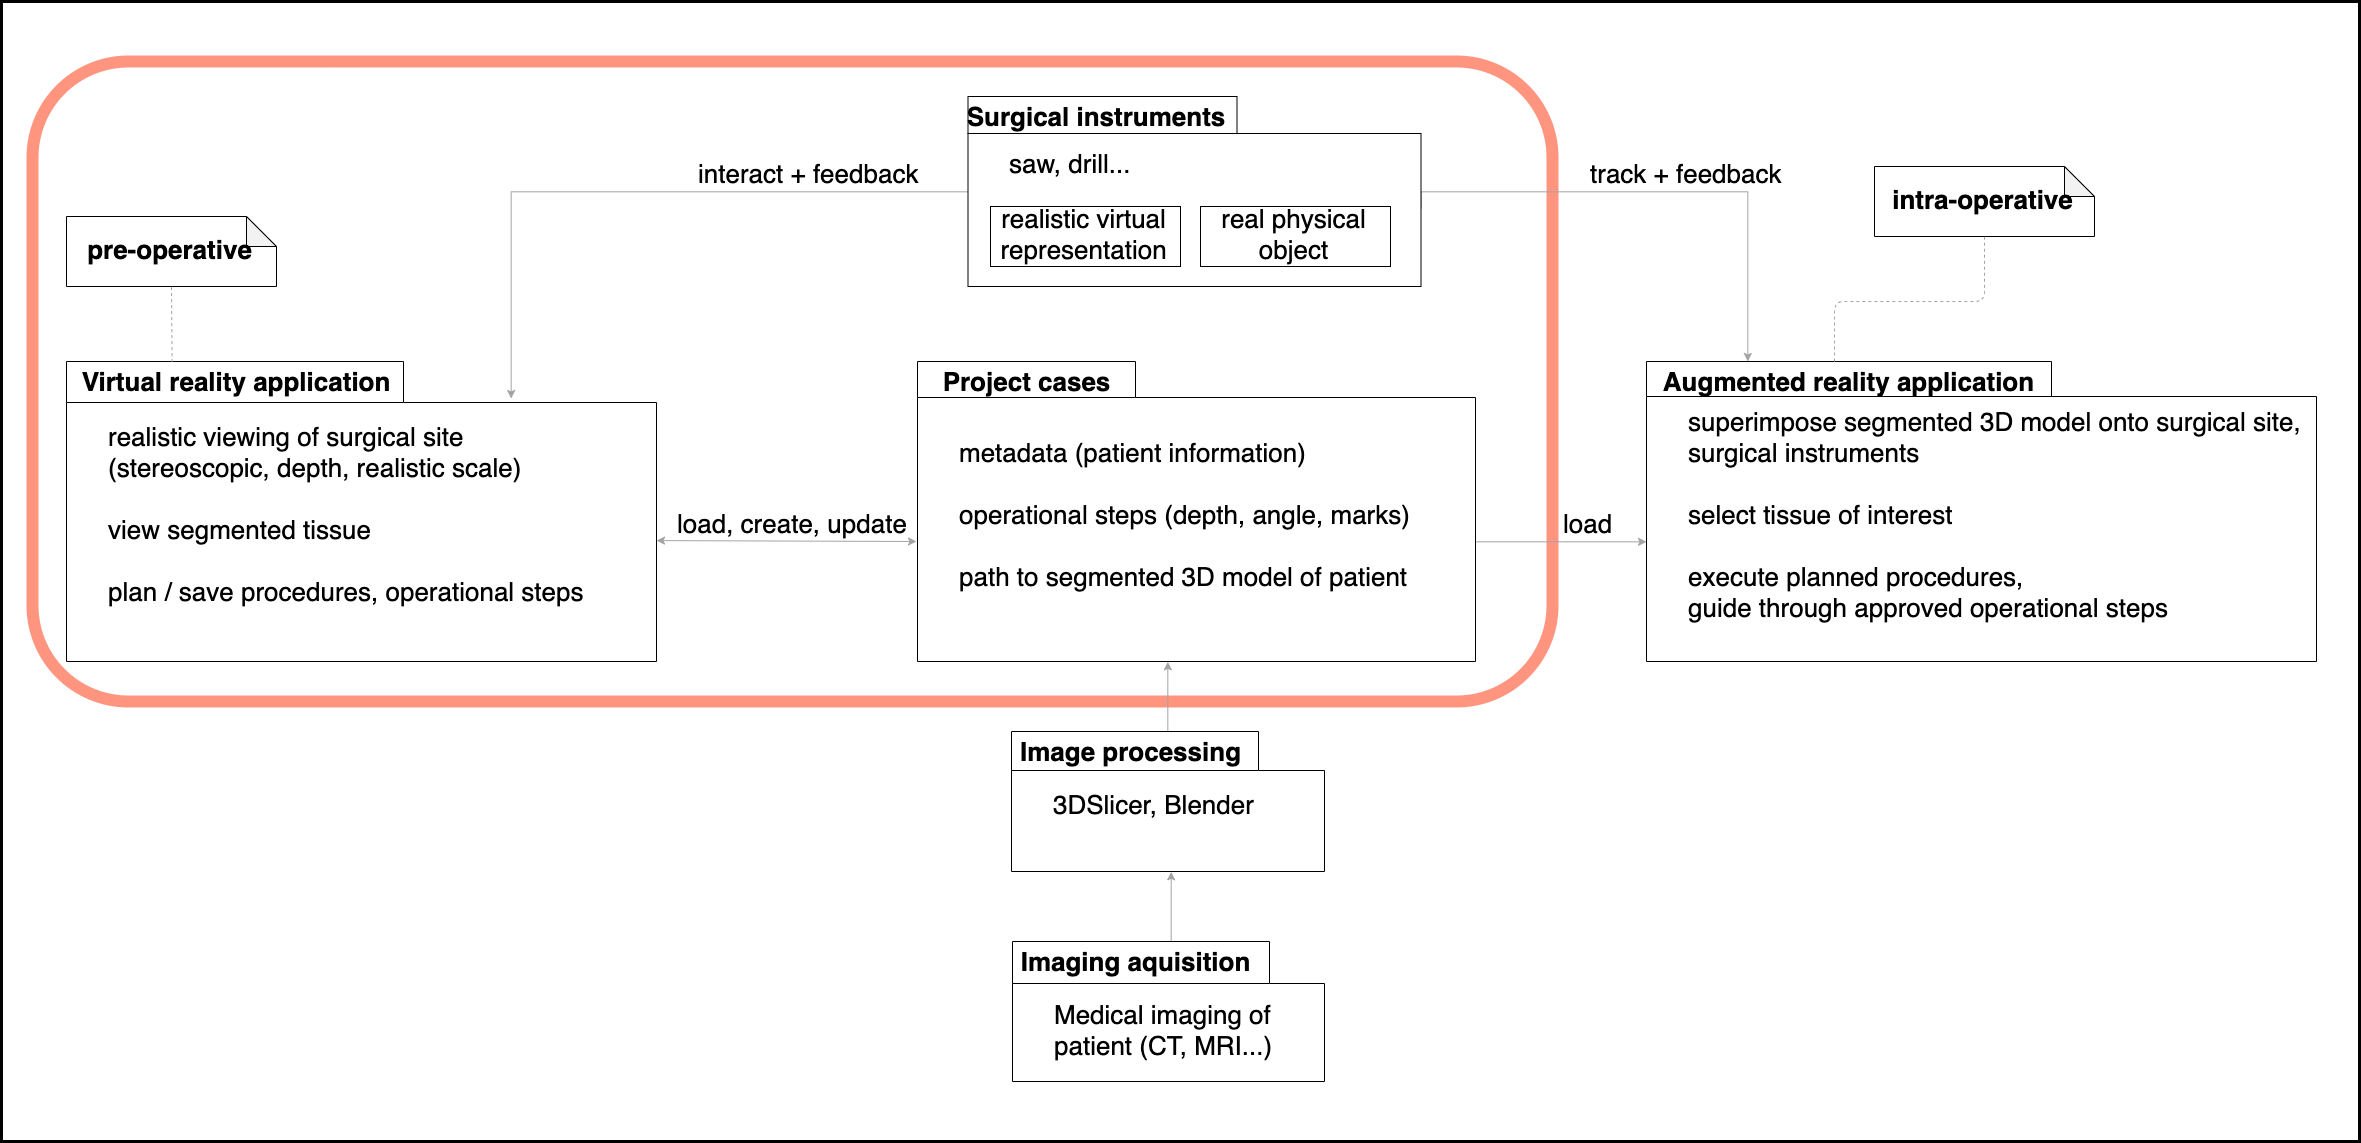
\includegraphics[width=\linewidth]{images/project_plan.png}
    \caption{\label{fig::ProjectPlan} Complete concept for a VR-AR-based workflow for surgeons. The scope of the thesis is framed in red.}
\end{sidewaysfigure}
Planned steps should be storable in a format in which they can be loaded and viewed in both the VR and AR applications bi-directionally as described (Figure \ref{fig::ProjectPlan}).
A JSON-notation has already been agreed and decided upon in the conceptualization phase of the project, since it is critical for a smooth 
interaction in the VR-AR-based workflow.
\\ A common storage format in form of a project case was designed and is utilized for both projects in the VR-AR workflow.
Project cases will store data about the case, such as patient information, finding, and planned steps, in text format.
To enable easier sharing of project cases, the patient's 3D model will be stored on user's hard drives and the file location will be stored in the project case. 
This way, the original model can be retained simply by copying it the first time it is saved.
Additionally, modifications made to the patient's 3D model should be persisted so that they can be easily accessed by another VR or AR user. 
However, this will require some sort of run-time import and export of 3D models.

In contrast to the presented work, this thesis aims to provide a useful tool not only for learning, but also for planning patient specific surgeries.
Because of technology advancing rapidly, VR and AR become more and more affordable options.
Mentioned limitations in regards to performance for high resolution patient specific 3D models are not an issue anymore.
\\ By using patient anatomy and pathology specific models, surgeons can profit from the mentioned benefits of VR simulation not only as a learning tool.
Moreover, the goal is to give trained surgeons a useful system which adds to the arsenal of existing planning techniques.
However, trainees can also benefit immensely by studying and reproducing planned procedures of experts.
\\ The first step in realizing these requirements is to develop a software architecture with an interface to the AR application in mind.
Since this is a bi-directional data exchange, which does not need to be real time, one obvious approach would be to use a simple object notation language such as JSON.
A humanly readable format should be used, so that operation plans can even be constructed without the need of an HMD.
\\ In principle, a procedure can be planned completely outside of the VR application in a 3D modeling application of choice, i.e. Blender 3D.
By creating appropriate geometry and adding them as steps to the patient's model, a complete project case can be created.
Then, the project case can be viewed, or "played" step by step as a training and visualization tool in VR as well as AR.
\\ Although possible, the preferred way of planning should be utilizing the VR applications' advantages.
In an immersive virtual OT, users will be able to plan and train surgical procedures for OMFS.
Many tools which are used in real procedures during surgery in the OMFS department of the UHA will be available to the user to plan procedures.
Any of those tools could be used to add procedure steps to the project case.
\\ Moreover, by planning the operational steps in VR, planned procedures can easily be shown to other staff involved by simply sharing the project cases.
Naturally, it will be of uttermost importance that medical equipment and an appropriate virtual environment is recreated remarkably close to reality in the VR application.
In addition, contrary to the AR part of the workflow, in VR users should be able to either create steps for the project case or modify existing ones.